\documentclass[a4paper,12pt]{article}
\usepackage[utf8]{inputenc}
\usepackage[T1]{fontenc}
\usepackage[hungarian]{babel}
\usepackage{graphicx}
\usepackage{geometry}
\geometry{a4paper,
		     tmargin = 30mm, 
		     lmargin = 30mm,
		     rmargin = 30mm,
		     bmargin = 30mm}
\usepackage{mathtools}
\usepackage{amsmath}
\usepackage{color}
\usepackage{setspace}
\usepackage{amsmath,amssymb}
\usepackage{float}
\usepackage{indentfirst}
\usepackage{algorithm}
\usepackage{algorithmic}
\usepackage{setspace}

\usepackage{natbib}

\renewcommand\thesection{\Roman{section}}
\renewcommand\thesubsection{\thesection.\arabic{subsection}}

\begin{document}

\begin{titlepage}

	\centering
	
	
\includegraphics[width=0.66\textwidth]{elte.jpg}
	\par\vspace{1cm}
	{\scshape\LARGE ELTE TTK \par}
	{\scshape\large Fizika szak \par}
	\vspace{1cm}
	
	{\scshape\LARGE Szakdolgozat \par}
	\vspace{1cm}
	
	{\scshape\Large Koaleszcencia modell kidolgozása transzportmodellekhez\par}
	\vspace{0.2cm}
	{\Large\itshape Olar Alex\par}
	\vspace{2cm}
	
	témavezető\par
	\vspace{0.3cm}
	{\Large Wolf György}

	\vfill

	{\large 2018 \par}
	
\end{titlepage}

\onehalfspacing

\begin{abstract}
\par Egy nehézion ütközésben résztvevő alkotó elemek száma néhány ezerig terjed legfeljebb, így a kidolgozott néhány-test elméletek, mint a három-test problémára kidolgozott Fagyejev-egyenletek \cite{fagyejev}, nem alkalmazhatóak, de az alkotóelemek alacsony száma miatt még a statisztikus fizikai modellek sem használhatóak, ráadásul nem is egyensúlyi reakciókról van szó az esetek többségében.
\vspace{5mm}
\par A rendelkezésre álló számítási kapacitás lehetővé tette, egy-egy ilyen nem egyensúlyi reakció teljes vizsgálatát, mikroszkopikus transzport-modellek segítségével. Egy ilyen modell a Boltzmann-Uehling-Uhlenbeck elmélet (BUU), ami fázistérben leírja adott részecskék között az ütközéseket és figyelembe veszi az azok között ható kölcsönhatást, egy időfüggő, átlagtér potenciállal. Korai modellek a részecskéket szabadnak tekintették, amikor azok nem vettek részt ütközésekben.
\vspace{5mm}
\par Az én célom, hogy egy, a BUU-ra épülő szimulációhoz \cite{wolfDSC} kidolgozzak egy olyan programot, ami a kölcsönható részecskéket, esetemben főként nukleonokat, klaszterezi, azaz csomósodásokat keres különböző távolság definíciók mellett (térben, impulzustérben, stb.). Ennek fontos szerepe lehet a detektor válasz meghatározásakor, valamint a darmstadti, CBM/FAIR projekt keretében szükség lesz az egyszeres és kétszeres ritkaságú magok keltésének vizsgálatára. Egyszeresen ritka magokat már találtak, de a kétszeres ritkaságúak modellezése nagyon fontos lehet a jövőben.
\end{abstract}

\vfill

\newpage
\tableofcontents
\newpage

\section{Elméleti áttekintés}

\subsection{Bevezető}

\par Egy nehézion ütközés, erősen nem egyensúlyi, erősen kölcsönható rendszer. A statisztikus fizikában $N > 10^{23}$ részecskére jól kidolgozott, statisztikus modell áll rendelkezésünkre, továbbá lehet magyarázni a néhány részecske rendszereket is, azonban például egy $Au+Au$ ütközésben a részecskék száma még és már nem kezelhető a korábbi modellekkel.

\vspace{5mm}

\par Kezdetben a folyamat leírására termodinamikai modelleket állítottak fel, amelyekben különböző hipotézisekkel éltek a nem egyensúlyi rendszerre vonatkozólag. Ezek közé tartozott, hogy a részecskék gyorsan termalizálódnak és kialakul egy globális egyensúly, és már egyensúlyi állapotukban detektáljuk őket. Ezután hidrodinamikai modellekhez folyamodtak amelyekben már nem volt globális, csak lokális termodinamikai egyensúly.

\vspace{5mm}

\par Azonban egy prominensebb ága a nehézion ütközések leírásának a nem egyensúlyi, mikroszkopikus transzport-modellek \cite{trs}. Először kaszkád elméleteket dolgoztak ki, amelyben a részecskék csak ütközéskor hatottak kölcsön, később azonban hosszú hatótávolságú erőket és nukleáris potenciálokat is figyelembe vettek.

\vspace{5mm}

\section{Transzport-egyenletek}

\par A nehézion ütközések dinamikáját transzport egyenletek segítségével lehet vizsgálni. Ennek két fő irányzata van, az egyik a Boltzmann-modellre épülő hidrodinamikai megközelítés, ami szerint 

\vspace{5mm}

\begin{equation}
	N = \int d^{n}\vec{p} \int d^{n}\vec{q} \quad f(\vec{q}, \vec{p}, t)
\end{equation}

\vspace{5mm}

ahol N a részecskék száma, míg $f(\vec{q}, \vec{p}, t)$ a fázistérben vett sűrűség függvény. Mivel a fázistérfogat elem ( $d^{n}\vec{p}\cdot d^{n}\vec{q}$ ) állandó, azonban ütközés során a részecske sűrűség változik, így az csak a fázissűrűségen keresztül változhat. Így tehát kapjuk a Boltzmann-egyenletet \cite{wolfDSC, buuEq}, amit a Liouville-tételből származtathatunk

\vspace{5mm}

\begin{equation}
	\frac{df}{dt} = \frac{\partial f}{\partial t} + \sum_{i = 1}^{n}\Big(\frac{\partial f}{\partial p_{i}}\frac{dp_{i}}{dt} + \frac{\partial f}{\partial q_{i}}\frac{dq_{i}}{dt}\Big) = I_{coll}
\end{equation}

\vspace{5mm}

\par Ezt pedig a szokott alakra hozva, bevezethetünk egy $I_{coll}$ \cite{wolfDSC} ütközési integrált, amire különböző hipotéziseket tehetünk majd fel.

\vspace{5mm}

\begin{equation}
	\frac{df}{dt} = \frac{\partial f}{\partial t} + \sum_{i = 1}^{n}\Big(\frac{\partial f}{\partial q_{i}}\frac{\partial H}{\partial p_{i}} - \frac{\partial f}{\partial p_{i}}\frac{\partial H}{\partial q_{i}}\Big) = I_{coll}
\end{equation}

\vspace{5mm}

\par Ez még természetesen csak az alapvető fizikai modell, a transzport-modellhez az úgynevezett Boltzmann-Uehling-Uhlenbeck \cite{buu} egyenleteket használják. Tehát az előbbi egyenletbe bevezetnek egy impulzusfüggő átlagteret $U(\vec{q}, \vec{p})$. Alacsony energiákon a rugalmatlan ütközések elhanyagolhatóak, a rendszer csak nukleonokból áll. 

\vspace{5mm}
	
\begin{gather}
	m^{*}(\vec{q}, \vec{p}) = m_{N} + U(\vec{q}, \vec{p}) \quad \quad E^{2} = m^{* 2} + p^{2} \\ 
	\frac{\partial H}{\partial q_{i}} = -\frac{dp_{i}}{dt} \quad \quad \frac{\partial H}{\partial p_{i}} =\frac{dq_{i}}{dt}
\end{gather}

\vspace{5mm}
	
\par Ahol tömeghéjon lévő kvázi-részecske közelítéssel élve az egyenlet átfogalmazható, felhasználva a Hamilton-egyenleteket:

\vspace{5mm}

\begin{equation} \label{BUU-eq:1}
	\frac{\partial f}{\partial t} + \frac{\partial f}{\partial \vec{p}}\Big(-\frac{m^{*}}{E}\nabla_{\vec{q}}U\Big) + \frac{\partial f}{\partial \vec{r}}\Big(\frac{\vec{p}}{E}+\frac{m^{*}}{E}\nabla_{\vec{p}}U\Big) = I_{coll}
\end{equation}

\vspace{5mm}

\par Az ütközési integrál ( $I_{coll}$ ) kvantumos jelenségek közül csak a Pauli-elvet veszi figyelembe, így jelentős részben klasszikus fizikán alapszik. Az így kapott egyenletet \eqref{BUU-eq:1} Boltzmann-Uehling-Uhlenbeck-egyenletnek nevezik, ha az ütközési integrállá feltesszük, hogy az $f(\vec{q}, \vec{p}, t)$ függvény időfejlődését írja le két-test kölcsönhatások hatására. 

\vspace{5mm}

\par Az $f(\vec{r_{1}}, \vec{p_{1}}, t)$ függvényt véve, valamint a $\vec{p}_{1} + \vec{p}_{2} \longleftrightarrow \vec{p}_{3} + \vec{p}_{4}$ ütközést vizsgálva az ütközési integrál a következő alakot veszi fel:

\vspace{5mm}

\begin{equation}
\begin{split}
I_{coll} = \frac{g}{(2\pi)^{3}}\int d^{3}p_{2}\int d^{3}p_{3}\int \Omega_{4}v_{12}\frac{d\sigma_{12 \rightarrow 34}}{d\Omega}\delta(\vec{p}_{1} + \vec{p}_{2} - \vec{p}_{3} - \vec{p}_{4})\cdot\\
\cdot(f_{3}(\vec{r}, \vec{p_{3}}, t)f_{4}(\vec{r}, \vec{p_{4}}, t)\bar{f}_{1}(\vec{r}, \vec{p_{1}}, t)\bar{f}_{2}(\vec{r}, \vec{p_{2}}, t) \\
- f_{1}(\vec{r}, \vec{p_{1}}, t)f_{2}(\vec{r}, \vec{p_{2}}, t)\bar{f}_{3}(\vec{r}, \vec{p_{3}}, t)\bar{f}_{4}(\vec{r}, \vec{p_{4}}, t))
\end{split}
\end{equation}

\vspace{5mm}

\par Ahol $\frac{d\sigma_{12 \rightarrow 34}}{d\Omega}$ a differenciális nukleon-nukleon hatáskeresztmetszet közegben, $v_{12}$ a nukleonok közötti relatív sebesség, valamint $\bar{f}$ függvény a Pauli-kizárási faktorok $1 - f$ módon állnak elő. Az integrál lényegében azt fejezi ki, hogy az $p_{1},p_{2}$ impulzusú nukleonok, ha ütköznek, akkor hogyan változhat meg az impulzusok $p_{3}, p_{4}$-re és fordítva. A harmadik, $d\Omega_{4}$-re vett integrál lényegében $d^{3}p_{4}d\Omega$ integrál, csak a differenciális hatáskeresztmetszet a szemléletes kép miatt le van választva.

\vspace{5mm}

\subsection{ Numerikus megoldás}

\vspace{5mm}

\par A témavezetőm szimulációs kódja \cite{wolf3, wolf2} a szokásos módszerrel áll neki ennek az integro-differenciál egyenlet megoldásának. A folytonos eloszlásfüggvény helyettesíthető véges számú pontrészecskékkel, matematikailag Dirac-delta disztribúciókkal. A fluktuációk simítása érdekében $N$ párhuzamos eseményt vizsgálva az eloszlás függvény $A$ nukleonra:

\vspace{5mm}

\begin{equation}
	f(\vec{r}, \vec{p}, t) = \frac{1}{N}\sum_{i}^{N \times A} \delta(\vec{r} - \vec{r}_{i}(t))\delta(\vec{p} - \vec{p}_{i}(t))
\end{equation}

\vspace{5mm}

\par Ezt bevezetve látható, hogy a modell leegyszerűsödött pontrészecskék mozgására. A mozgásegyenletek a Hamilton-egyenletekből kaphatóak, amelyeket a \eqref{BUU-eq:1}-ben is felhasználtam. A potenciál, sűrűségek és a Pauli-effektus számolásánál a pontrészecskék Gauss-eloszlásokkal vannak helyettesítve \cite{wolfDSC}.

\vspace{5mm}

\par A transzport-modell nem tartalmaz szabad paramétereket. A deriváltakat differenciálok váltják fel. Az egy-részecske mozgásegyenlet megoldásához a prediktor-korrektor módszer a következő:

\vspace{5mm}

\begin{gather}
	\vec{p}^{pr}_{i} = \vec{p}_{i} - \Delta t \frac{\partial H}{\partial \vec{r}_{i}} \quad \quad \vec{r}^{pr}_{i} = \vec{r}_{i} + \Delta t \frac{\partial H}{\partial \vec{p}_{i}}
\end{gather}

\vspace{5mm}

\par Ahol $^{pr}$ jelöli a prediktált helyet és impulzust. Ez még korrekcióra szorul, ehhez ki kell számolni az prediktált helyen a Hamilton-függvény értékét, majd a helyet és momentumot annak megfelelően léptetni

\vspace{5mm}

\begin{gather}
	\vec{p}^{co}_{i} = \vec{p}_{i} - \frac{\Delta t}{2} \Big(\frac{\partial H}{\partial \vec{r}_{i}} + \frac{\partial H^{pr}}{\partial \vec{r}_{i}^{pr}} \Big) \quad \quad \vec{r}^{co}_{i} = \vec{r}_{i} + \frac{\Delta t}{2} \Big( \frac{\partial H}{\partial \vec{p}_{i}} + \frac{\partial H^{pr}}{\partial \vec{p}_{i}^{pr}} \Big)
\end{gather}

\vspace{5mm}

\par Az átlagtér potenciált úgy kell választani, hogy az anyag összenyomhatóságát jól jellemezze. Néha, az eredményekkel való összehasonlítási céllal ki szokták hagyni az impulzus függést is.

\vspace{5mm}

\section{ Koaleszcencia}

\vspace{5mm}

\par Az én feladatom a kimeneten szolgáltatott, térbeli és impulzustérbeli részecskeeloszlások alapján az volt, hogy egy olyan eljárást dolgozzak ki, amivel vizsgálható lesz a detektorválasz és a későbbiekben akár egyszeresen és kétszeresen ritka magok keltése. Lévén, hogy nukleonokra koncentráltam, a kimenetek közül is egyenlőre ezeket vizsgáltam. A koaleszcencia \cite{koleszcenciaSato} modell lényege, hogy a nukleonok ha elegendően közel kerülnek egymáshoz impulzustérben, akkor bizonyos valószínűséggel összetapadnak és a detektorban már csak egy beütés észlelhető így, több összetapadt, töltéssel rendelkező részecske esetén.

\vspace{5mm}

\par A mechanizmust amely a nehézion-ütközések után kialakuló közepes méretű magokat leírja többen is megpróbáltak leírni. A koaleszcencia modell részletes leírása deuteron esetén megtalálható $J. I. Kapusta$ cikkében. A szakirodalom a közepes magokkal foglalkozik (Z $\leq$ 12 \cite{REISDORF1997493}), ezeket az angol rövidítés alapján $IMF$\footnote{intermediate fragments}-nek nevezem majd. 

\vspace{5mm}

\par $Kapusta$ \cite{kaposzta} arról ír, hogy bármikor, amikor egy neutron és proton kellően közel kerül egymáshoz, azaz impulzusok egy $p_{0}$ gömbön belül van, valamint a megfelelő spinállapotban vannak, akkor összetapadnak. A spin- és izospin-állapotokat figyelmen kívül hagyva, én is a minimális távolság alapján implementáltam a koaleszcenciát, később azonban végzek majd szűrést a ténylegesen kialakuló, természetben előforduló magokra. A modell térben és impulzustérben is tud, külön-külön, a kettő együttesét a mérési adatokra megfelelően választott súlyfaktorokkal lehet implementálni.

\vspace{5mm}

\par Azért a deuteronra került a legnagyobb hangsúly, mert lényegében csak az ütközés termékeként keletkezhet és nem lökődik ki a keletkezett magokból, mint például az $\alpha$-részecske. Tehát az esemény (nehézion-ütközés) dinamikája lényegében megmutatkozik a deuteron magokban. A \cite{kaposzta} - cikkben lényegében a deuteronok számsűrűségére a következő feltevéseket teszik

\vspace{5mm}

\begin{itemize}
\item legyen $\gamma \frac{d^{3}n_{N}}{dp^{3}}$ a relativisztikusan invariáns impulzustérbeli sűrűség nukleonokra
\item protonokra és neutronokra ugyan azt a sűrűséget tételezi fel, de könnyen módosítható nem azonos sűrűségekre
\item $\vec{p}$ impulzus körül egy $p_{0}$ sugarú gömbben egy nukleon megtalálásának valószínűsége $P = \frac{1}{M}\frac{4\pi}{3}p_{0}^{3}\gamma \frac{d^{3}n_{N}}{dp^{3}}$, ahol $M$ a nukleonok átlagos száma
\item ha ez a valószínűség kicsi, és M kellően nagy, akkor a deuteronra (binomiális statisztika miatt) $\gamma \frac{d^{3}n_{d}}{dp^{3}} = \frac{1}{2}\frac{4\pi}{3}p_{0}^{3}(\gamma \frac{d^{3}n_{N}}{dp^{3}})^{2}$
\end{itemize}

\vspace{5mm}

\par Itt $p_{0}$ később a klaszterező paraméterem lesz, melynek értékét a klaszterek számának változásából fogom meghatározni. Ahol a klaszterek száma drasztikusan csökkenni kezd, olyan tartományban érdemes majd az $IMF$-eket keresni. Ezen koaleszcenciának nagy előnye, hogy rendkívül általános és nem tételez fel semmit a rendszer mechanizmusairól.

\vspace{5mm}

\subsection{ Szélességi bejárás - Breadth-first Search (BFS)}

\par A szélességi bejárás egy jól ismert gráf algoritmus az informatikában \cite{bfs}. Az algoritmus lényege, hogy egy gráfban adott tulajdonságú pontot keresve kiválogassa azt, biztosítva, hogy minden csúcsot leellenőrzött. Én nem egészen erre használom, mivel nekem klaszterezésre van szükségem, tehát nem adott tulajdonság alapján kell kiválogatnom csúcsokat, hanem egy nem összefüggő gráfot kellett darabjaira szétszednem.

\vspace{5mm}

\par Így az algoritmust kicsit módosítanom kellett. Hasznos tulajdonságai közé tartozik, hogy gyors, és biztosítja, hogy minden elemén a gráfnak végigmegy. Így tehát addig kell ismételgetnem az algoritmust egy nem összefüggő gráfon míg annak vannak csúcsai összefüggő részgráfokban. 

\vspace{5mm}

\par Az algoritmus kiválaszt egy kezdőcsúcsot, majd a csúcsokat látogatottság szerint besorolja. Ezután egy szomszédsági lista szerint végigjárja az adott csúcs szomszédait. Lényegében ez a klaszterek megkeresésének módja. Hiszen miután kifogy a szomszédsági lista, kiválasztható véletlenszerűen egy újabb csúcs, amin elindulva szintén megtalálhatóak annak szomszédai. 

\vspace{5mm}

\par A pszeudokódot mellékelem, hiszen az alapimplementáció C++, majd Fortran nyelveken valósul(t) meg.

\vspace{5mm}

\begin{center}
\begin{algorithm}
\caption{BFS klaszterező függvény}
\begin{algorithmic}
\STATE visitedVertices = vector($bool$)[FALSE]
\STATE startingVertex = 0
\WHILE{ allVerticesVisited(visitedVertices) }
	\STATE cluster = vector()
	\STATE visitedVertices[startingVertex] = TRUE
	\STATE queuedVertices = Queue()
	\STATE queuedVertices.Queue(startingVertex)
	\WHILE{ queueIsNotEmpty(queuedVertices) }
		\STATE currentVertex = queuedVertices.Front()
		\FORALL{ element of adjecencyList[currentVertex] }
			\IF{ isNotVisited(element) }
				\STATE visitedVertices[element] = TRUE
				\STATE queuedVertices.Queue(element)
			\ENDIF
		\ENDFOR
	\STATE saveCluster(cluster)
	\STATE startingVertex = findFirstNotVisited(visitedVertices)
	\ENDWHILE
\ENDWHILE
\end{algorithmic}
\end{algorithm}
\end{center}

\vspace{5mm}

\subsection{ Implementáció}

\par Mint ahogy az előző pontban említettem az algoritmushoz egy gráf szükséges. A szimuláció kimenetén a nehézion-ütközésekből nyert nukleonok hely- és impulzuseloszlását kapom meg. Mivel egy ütközés paralel $N$-szer lefut, egymás után pedig ez $M$-szer ismétlődik meg, így egy szimuláció során $N\cdot M$ kiértékelhető adatsort kapok, amikből már kellően nagy $N, M$ esetén már jó statisztikát lehet készíteni. Az eloszlások alapján térben és impulzustérben is szükségem van egy $r_{0}$ és egy $p_{0}$ klaszterező méretre. A bemeneti adataim $~fm~$ és $~GeV/c~$ nagyságrendűek. Egy klaszterdefiniálásánál kihasználom a négyesimpulzus-megmaradást, 

\vspace{5mm}

\begin{equation}
	E = \sum_{i} E_{i} \quad \quad \vec{p} = \sum_{i} \vec{p}_{i}
\end{equation} 

\vspace{5mm}

\par ahol az összegzés a klaszterekben lévő részecskékre megy. Itt nem veszem figyelembe, hogy kötési energia szabadul fel, csak egy közelítést szeretnék adni a majdani sebességre

\vspace{5mm}

\begin{equation}
	p = \frac{v}{c} E \quad \quad E = \sqrt{M^{2} + p^{2}}
\end{equation}

\vspace{5mm}

\par A $M$ tömeg tisztán a klaszterben lévő nukleonok tömege, ahol a proton tömegét $0.938 ~Gev/c$-nek, míg a neutron tömegét közelítőleg $0.939 ~Gev/c$-nek vettem. Az impulzus a fentebbi képlet alapján adott volt. Az irodalomban több helyen is elhanyagolják teljes mértékben a térbeli koaleszcenciát lévén, hogy relativisztikus részecskékről van szó, és az impulzustérbeli szomszédság így sokkal tovább fennáll, mint a térbeli.  

\vspace{5mm}

\par A programom beolvassa a $K$ számú adatfájlt, melyekből klasztereket csinál a $BFS$ algoritmus segítségével, valamint elvégzi a szükséges számításokat és ezek után egy fájlban kiadja a klaszterméretet, energiát, sebességet, impulzuseloszlást és a kirepülő részecskék polárszögét.

\vspace{5mm}

\begin{equation}
\varphi = \arccos\Big(\frac{p_{x}}{\sqrt{p_{x}^{2} + p_{y}^{2}}}\Big)
\end{equation}

\vspace{5mm}

\section{ Mérési adatok}

\par A centrális arany-arany ütközéseket többek között a GSI-ben, Darmstadtban is vizsgáltak a FOPI kollaboráció keretében. A név egy $4\pi$ ('four pi') térszögű detektorra utal. Azaz ebben az elrendezésben a fragmentáció nagyon jól vizsgálható, hiszen minden irányban detektálni lehet a nehézion ütközések utána részecskéket. A FOPI-nál vizsgált nehézion nyalábot egy, a detektorban található céltárgyra bocsátották. Az általam használt szimulációban én be tudtam állítani, hogy az ütközéseim centrálisak legyenek, azonban a FOPI mérései során ezeket az eseményeket szűrni kellett, hiszen átlagosan $1\%$-át képviselték az összes ütközésnek.

\vspace{5mm}

\par Erre találták ki az $ERAT$ nevezetű mennyiséget. Ezt a következőképpen definiálták

\vspace{5mm}

\begin{equation}
ERAT = \frac{E_{t}}{E_{l}} = \frac{\sum_{i} p_{t,i}^{2}/(m_{i} + E_{i})}{\sum_{i} p_{l,i}^{2}(m_{i} + E_{i})}
\end{equation}

\vspace{5mm}

\par ahol $l,t$ indexek longitudinális és transzverzális energiákra és impulzusokra vonatkoznak. Az ütközés $z$-irányú, az összegzés a létrejött magokra megy. Az elv az, hogy feltétezik, hogy transzverzális energia túlnyomó többségében nukleon-nukleon kölcsönhatásból származik, és akkor maximális ha az ütközésben résztvevő magok a lehető legjobban átfednek, azaz ha centrális az ütközés. Ezt a mennyiséget nekem nem volt célszerű használnom, hiszen a generált eseményeim mind centrálisak voltak. Azonban jó indikátora lehet általános ütközéseknél a centrális eseményeknek.

\vspace{5mm}

\par Egy kizárólag termikus modell egy $T$ hőmérsékletű tágulás során tömegszám függvényében konstans energiát jósolnak ($\frac{3}{2}k_{B}T$), azonban, ha feltételezzük, hogy ütközés után egy izotrop robbanás megy végbe (az ősrobbanás analogonjára), akkor az egyes kirepülő nukleonoknak, egyenként van $\frac{3}{2}k_{B}T$ mozgási energiája, míg ha összetapadnak, akkor ez az energia a tömegszámmal kell arányos legyen

\vspace{5mm}

\begin{equation}
\big<E_{kin}\big> = a + b\cdot A_{f}
\label{blast-model}
\end{equation}

\vspace{5mm}

\begin{center}
\begin{tabular}{|c|c|c|c|c|}
\hline
E [A MeV] & b [GeV] & a [GeV] & $\Delta$b [GeV] & $\Delta$a [Gev] \\
\hline
250 & 0.056 & 0.179 & 0.004 & 0.060 \\
\hline
\end{tabular}
\end{center}

\vspace{5mm}

\begin{figure}[H]
\centering
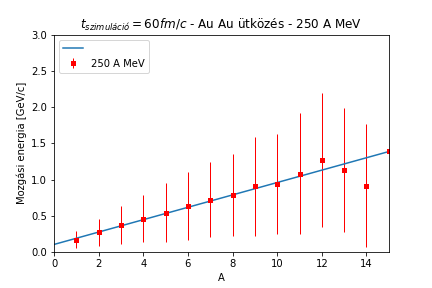
\includegraphics[width=0.75\textwidth]{./60fmcAuAu250AMeV007mom.png}
\caption{60 fm/c szimulációs idő, a vízszintes tengelyen a klaszterezett magok tömegszáma, míg a függőleges tengelyen a számolt mozgási energiájuk, $p_{0} = 70 ~MeV/c$ klaszterező paraméteren}
\end{figure}

\vspace{5mm}

\par Az alábbi ábrán látható, hogy csak [0;15] tömegszám intervallumban ábrázoltam a klaszterezett magokat, hiszen a FOPI mérés alapján ezek, az úgynevezett közepes magok (IMF) összehasonlíthatóak az én eredményeimmel is. A FOPI mérés adatai \cite{REISDORF1997493, SANTINI2005468} alapján tudtam összehasonlítani a sajátommal.

\vspace{5mm}

\par A készített ábráim és adataim az ő mérési és szimulációs eredményeiket akarja reprodukálni, hogy később ezt be lehessen építeni a hazai kódba. Így a detektor válasz nagyban jósolható lesz bizonyos atommagok ütközése esetén, valamint a későbbiekben egyszeresen és kétszeresen ritka magokat lehet majd szimulálni.

\vspace{5mm}

\par A FOPI-nál $150, 250$ és $400 ~A MeV$-en végeztek méréseket és modellezték azokat \cite{REISDORF1997493}. Az eredményeik között multiplicitáseloszlást vizsgáltak, nagyon kis rendszámú magok energiáit ($ Z = 1,2$), a kirepülő fragmentumok szögeloszlását, energiaeloszlását, valamint különböző polárszögeknél tömegszám szerinti eloszlásokat is, hogy ezekből jóslást tudjanak adni az ütközés dinamikájára. Ezen kívül vizsgáltak még a kirepülő klaszterek kémiai összetételét is. 

\section{ Eredmények}

\vspace{5mm}

\subsection{ Klaszterező paraméter}

\vspace{5mm}

\par Először is fontos vizsgálni, hogy milyen klaszterező méretet érdemes venni, amelyet általánosan használni lehet a különböző energiákon. Mivel a klaszterezést impulzus térben végeztem, $p_{0}$ értékét $(10 - 200) ~MeV/c$ közé becsültem. Lényegesen e felett a klaszterezés nem működik, hiszen minden részecske elég közel van egymáshoz ahhoz, hogy összetapadjanak. 

\vspace{5mm}

\par Az alábbi ábrán jól látható, hogy az érdekes tartomány, ahol hirtelen elkezd leesni a klaszterek száma $(0.03 - 0.09) ~GeV/c$ környékén keresendő. Fontos megjegyezni, hogy egy részecske, akkor tekinthető a klaszter elemének, ha annak valamely eleméhez $p_{0}$-nál közelebb van. Ez a BFS klaszterezésből egyértelműen következik. 

\vspace{5mm}

\begin{figure}[H]
\centering
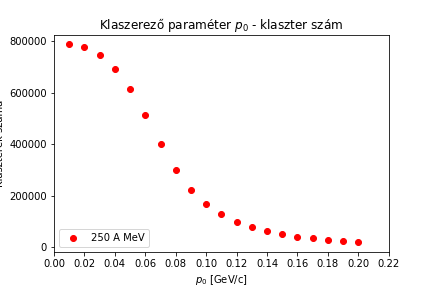
\includegraphics[width=0.75\textwidth]{./klaszterszamparameter.png}
\caption{250 A MeV-en, 2000 Au Au ütközésből készített klasztereken, különböző $p_{0}$ paraméterrel futtatott koaleszcencia}
\end{figure}

\vspace{5mm}

\par Kis $p_{0}$ paraméternél a klaszterek nagyon magas száma azért van, mert az algoritmusban nem szűröm ki az 1 nukleont tartalmazó 'klasztereket', hiszen később használom majd azokat az adatokat. Nagy $p_{0}$ esetén viszont látható, hogy néhány ezer klaszter van csak, ami természetes, hiszen néhány ezer magot ütköztetünk kezdetben.

\vspace{5mm}

\par A legjobb $p_{0}$ paraméter kiválasztásához a fentebbi adatsort lederiválva, azaz véve a diszkrét differencia értékeket a különböző klaszterező paraméterekre, azt a klaszterező paramétert választottam, ahol a 'legmeredekebb' az előző pontsorozat. Így itt most a derivált minimumát keressük. Az alábbi ábrán jól látható, hogy ez $p_{0} = 0.06 ~GeV/c$-nél van. A továbbiakban, hacsak külön ki nem emelem, akkor ezt fogom használni minden esetben. Természetesen ez egy szabad paramétere az algoritmusnak, így majd a tényleges gyakorlatban azt a $p_{0}$ paramétert kell venni, ami a legjobban visszaadja majd a kísérleti adatokat.

\vspace{5mm}

\begin{figure}[H]
\centering
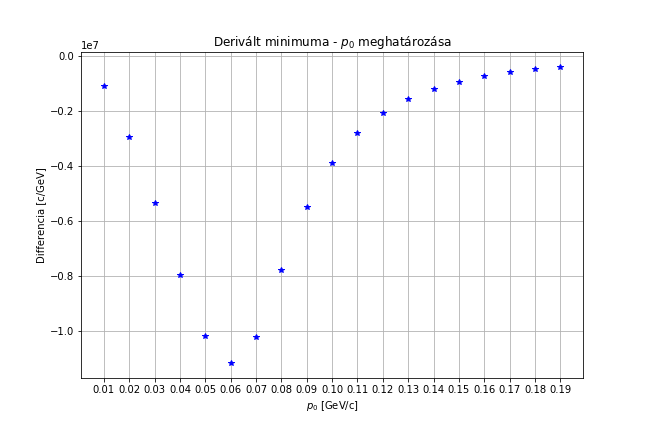
\includegraphics[width=0.85\textwidth]{./legjobb_p0.png}
\caption{250 A MeV-en, 2000 Au Au ütközésből készített klasztereken, különböző $p_{0}$ paraméterrel futtatott koaleszcencia, jól látható, hogy a minimum $0.06 ~GeV/c$-nél van}
\end{figure}

\subsection{ Közepes fragmentumok}

\vspace{5mm}

\par A FOPI által vizsgált $Z \in [0;12]$ az én statisztikáimban nem túl jó, hiszen én sokkal kisebb (1000-2000) körüli eseményszámmal dolgozom, míg náluk volt másod percenként $10^{5}$ nehézion ütközés, melynek $1\%$-át centrálisnak becsülték, azaz másodpercenként kaptam annyi adatot, mint amennyit én használtam. Azonban az én ütközéseim a szimuláció miatt biztosan centrálisak, ők viszont csak az $ERAT$ paraméterrel tudták a legbiztosabban besorolni az ütközéseket.

\vspace{5mm}

\subsubsection{ Különböző $p_{0}$ paraméterek}

\vspace{5mm}

\par A lenti ábrán jól látható, hogy ugyan azon az Au-Au ütközésen, különböző $p_{0}$ mellett futtatott klaszterezések során nincs $Z = 5$-nél nagyobb rendszámú mag, amely minden futtatás után biztosan jelen van. Látszik az is, hogy a klaszterek száma egyre jobban szór $Z$ növekedtével, azaz lényegében látszik, hogy a nagyobb magok kialakulása centrális ütközésekben egyre valószínűtlenebb.

\vspace{5mm}

\begin{figure}[!htb]
\centering
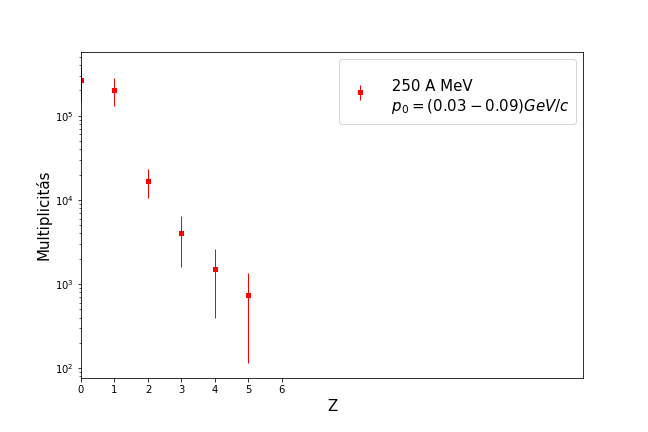
\includegraphics[width=0.75\textwidth]{./p0valtozik_klaszterek.png}
\caption{250 A MeV-en, 2000 Au-Au ütközésből készített klasztereken, $p_{0} = (30 - 90) ~MeV/c$ paraméterrel futtatott koaleszcencia}
\end{figure}

\vspace{5mm}

\subsubsection{ Különböző események, azonos $p_{0}$}

\vspace{5mm}

\par Ugyanolyan energiájú, centrális, azonos klaszterező paraméterű $Au-Au$ magok ütközése esetén viszont már sokkal megnyugtatóbb eredményt kaptam. Hiszen az előbb a klaszterező paramétertől való függés igen jelentős volt, azonban most, a klaszterek számának szórása és eloszlása nem változik jelentős mértékben különböző eseményekre. 

\vspace{5mm}

\begin{figure}[!htb]
\centering
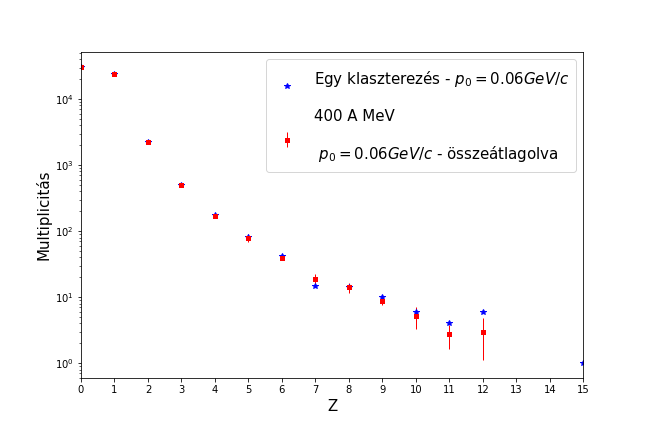
\includegraphics[width=0.8\textwidth]{./p0allando_kulonbozoRandom.png}
\caption{400 A MeV-en, 5*200 Au Au ütközésből készített klasztereken, $p_{0} = 60 ~MeV/c$ paraméterrel futtatott koaleszcencia, látható egy (csillag) ütközésre vett klaszterek eloszlása és 5 esemény összeátlagolva (négyzet)}
\end{figure}

\vspace{5mm}

\subsection{ FOPI mérések reprodukálása}

\vspace{5mm}

\subsubsection{ Koaleszcencia különböző energiákon}

\vspace{5mm}

\par Először ábrázoltam a multiplicitásokat, azonos klaszterező paraméter mellett, ez természetesen az előbb meghatározott $p_{0} = 60 ~Mev/C$, különböző ütközési energiákon. A legkisebb magokat kivéve $Z = 0, 1, 2, 3$ az adatsorból, a rendszám-multiplicitás párokra egy exponenciális függvényt illesztettem

\vspace{5mm}

\begin{equation*}
M = N\cdot e^{-\lambda\cdot Z}
\end{equation*}

\vspace{5mm}

\begin{center}
\begin{tabular}{|c|c|c|c|c|}
\hline
E [A MeV] & N & $\lambda$ & $\Delta$N & $\Delta\lambda$ \\
\hline
150 & 5131 & 0.357 & 1885 & 0.068 \\
\hline
250 & 10807 & 0.55 & 1604 & 0.027 \\
\hline
400 & 17127 & 0.976 & 2823 & 0.032 \\
\hline
\end{tabular}
\end{center}

\vspace{3mm}

\begin{figure}[H]
\centering
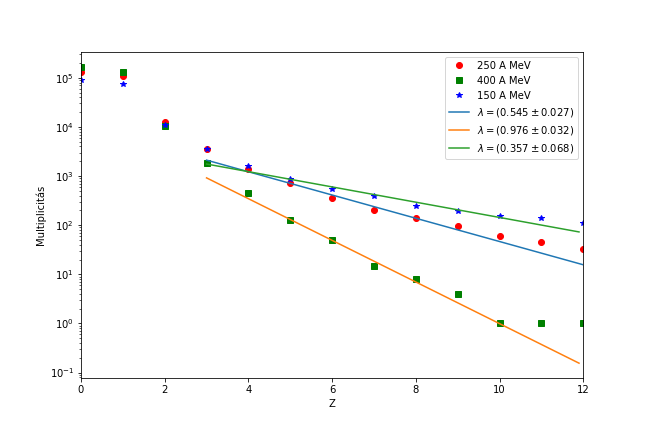
\includegraphics[width=0.8\textwidth]{./p006_250_400_fit.png}
\caption{150, 250 és 400 A MeV-en vett klaszterezésekre illesztett exponenciális függvények az adatsorokon, a $\lambda$ paraméter fel van tüntetve az illesztett függvényeken, $t_{\text{szimuláció}} = 60 ~fm/c$}
\end{figure}

\vspace{5mm}

\par Az illesztés csak $Z = 12$-ig megy, mivel ekkor tudtam a legszebb illesztést produkálni. A kisebb magok között és a nagyobb magok között is, nálam lehetnek számottevően neutrontöbbletes magok, melyeket én nem zárok ki a koaleszcencia során. Ez okozhatja, hogy az illesztés csak viszonylag kis tartományra működik jól. A későbbiekben végzek majd egy szűrést a periódusos rendszerben megtalálható magokra a pontosabb illesztés megtalálása végett.

\vspace{5mm}

\subsubsection{ Kis rendszámú magok }

\vspace{5mm}

\par A kis rendszámú magok, ezek között túlnyomó többségben, $^{4}He, ^{2}H, ^{3}He, ^{1}H$, jól jellemzik a folyamatot. A koaleszcencia-modell is lényegében kis rendszámú magokra van kimondva és elméletileg indokolva, csak ezt a felvetést próbáljuk minél szélesebben alkalmazni. 

\vspace{5mm}

\par A következő ábrák adott ütközésen belül keletkezett összes $Z = 1, 2$ magok eloszlását mutatja. Az ábrákon jelöltem adott energián az átlagos számát a részecskéknek és azok szórását is. Csak $\varphi \in [60^{\circ};90^{\circ}]$ polárszög közötti részecskéket vettem figyelembe, hogy összevethető legyen a munkám a \cite{REISDORF1997493}-ben szereplő adatokkal és ábrákkal.

\vspace{5mm}

\par Az ábrákon látható függvény a korábbi, mozgási energiára illesztett egyenes, amit ide áthoztam, hogy szemléltesse, hogy milyen mértékben térnek el a legkönnyebb magok mozgási energiái attól.

\vspace{5mm}

\begin{figure}[H]
\begin{minipage}{\textwidth}
\centering
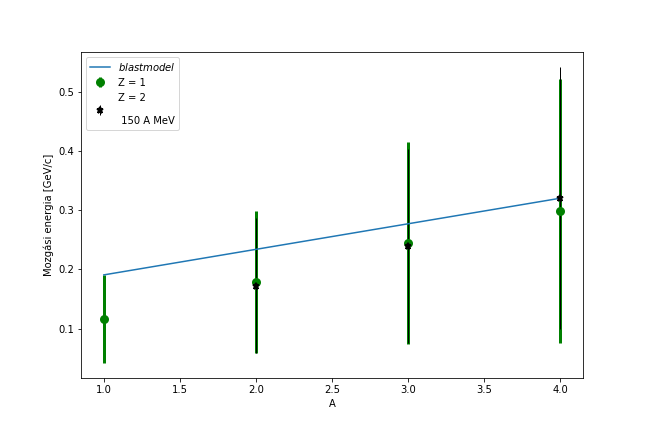
\includegraphics[width=0.67\textwidth]{./konnyu_magok_150AMeV.png}
\caption{150 A MeV-en vett könnyű magok eloszlása, $\varphi \in [60^{\circ};90^{\circ}]$}
\end{minipage}
\end{figure}
\begin{figure}[H]
\begin{minipage}{\textwidth}
\centering
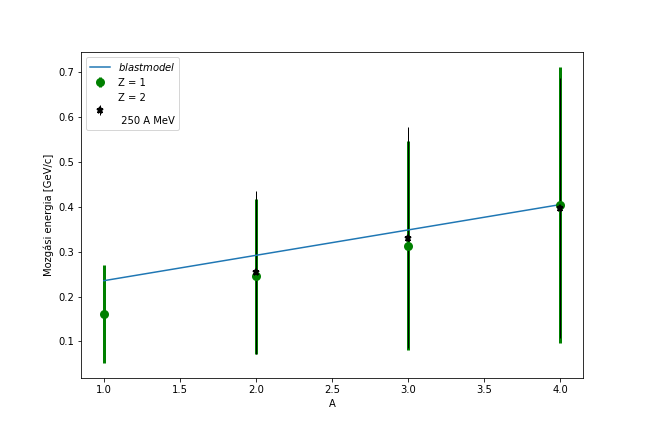
\includegraphics[width=0.67\textwidth]{./konnyu_magok_250AMeV.png}
\caption{250 A MeV-en vett könnyű magok eloszlása, $\varphi \in [60^{\circ};90^{\circ}]$}
\end{minipage}
\end{figure}
\begin{figure}[H]
\begin{minipage}{\textwidth}
\centering
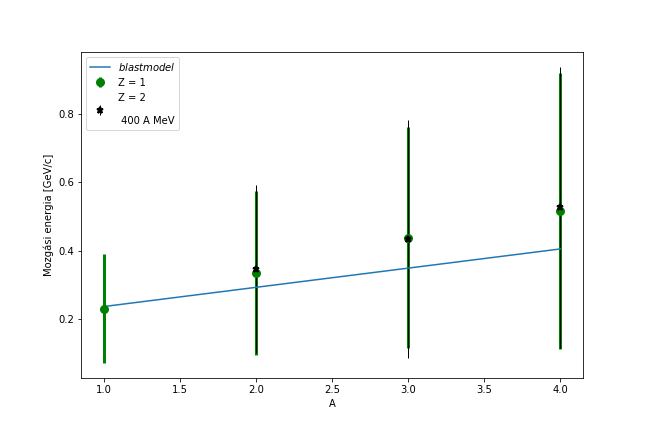
\includegraphics[width=0.77\textwidth]{./konnyu_magok_400AMeV.png}
\caption{400 A MeV-en vett könnyű magok eloszlása, $\varphi \in [60^{\circ};90^{\circ}]$}
\end{minipage}
\end{figure}

\vspace{65mm}

\subsubsection{ Izotrop robbanás}

\vspace{5mm}

\par Ahogy már a Mérési adatok című fejezetben már beszéltem róla, egy izotrop robbanásként kezelhető az ütközés utáni folyamat, ahol minden nukleonra $\frac{3}{2}k_{B}T$ energia jut, így a koaleszcencia után egyértelműen a tömegszámmal arányos kinetikus energiát vártam. Ezt szemlélteti a három ábrám, különböző energiákon. A pontok az egyes klaszterek átlagos energiáit jelölik, míg a függőleges vonalak azok szórását. Az illesztési paramétereket utána prezentálom, a (\ref{blast-model})-as egyenlet alapján.

\vspace{5mm}

\begin{figure}[H]
\centering
\begin{minipage}{.49\textwidth}
\centering
    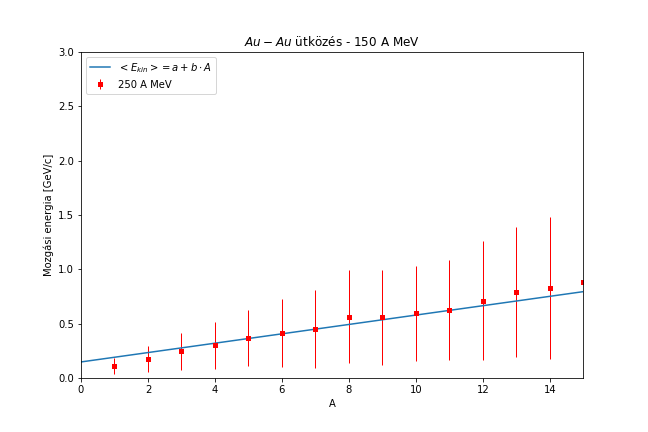
\includegraphics[width=\textwidth, height=\textwidth]{./150AMeV006mom2000adat.png}
    \caption{150 A MeV, $p_{0} = 60 ~MeV/c$}
\end{minipage}
\begin{minipage}{.49\textwidth}
\centering
    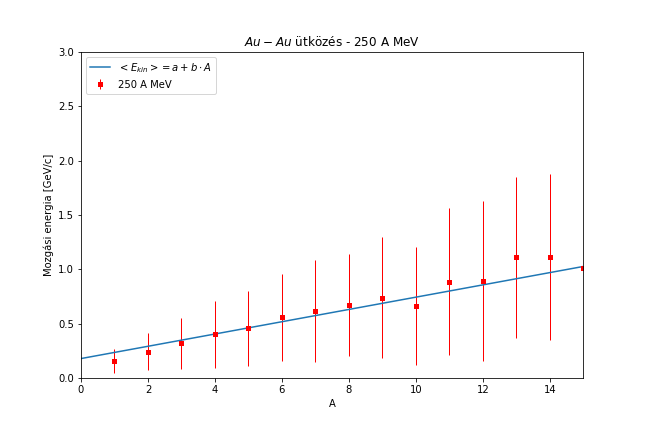
\includegraphics[width=\textwidth, height=\textwidth]{./250AMeV006mom2000adat.png}
    \caption{250 A MeV, $p_{0} = 60 ~MeV/c$}
\end{minipage}
\begin{minipage}[c]{.8\textwidth}
\centering
    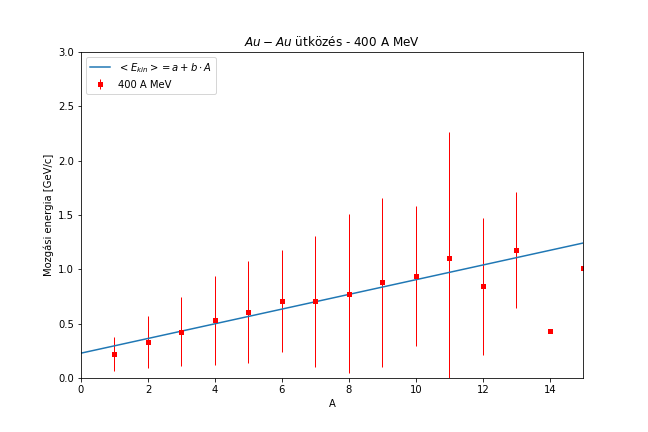
\includegraphics[width=\textwidth]{./400AMeV006mom2000adat.png}
    \caption{400 A MeV, $p_{0} = 60 ~MeV/c$, itt már a nagyobb magok kialakulás kisebb mértékű és a szórások is jócskán megnövekedtek}
\end{minipage}
\end{figure}

\par Az ábrák $\varphi \in [25^{\circ}; 45^{\circ}]$ polárszöget közötti magokat ábrázolnak. A [hivatkozás] cikkben ugyanezek megtalálhatóak. Az illesztési adatok pedig a következőek:

\vspace{5mm}

\begin{center}
\begin{tabular}{|c|c|c|c|c|}
\hline
E [A MeV] & b [GeV] & a [GeV] & $\Delta$b [GeV] & $\Delta$a [GeV] \\
\hline
150 & 0.043 & 0.148 & 0.001 & 0.016 \\
\hline
250 & 0.056 & 0.179 & 0.004 & 0.060 \\
\hline
400 & 0.068 & 0.228 & 0.006 & 0.046 \\
\hline
\end{tabular}
\end{center}

\vspace{5mm}

\par Az $a$ paraméter értéke különösen érdekes. Míg $E = 150 ~A MeV$-nél közel visszakapjuk az egy nukleonra jutó kezdeti mozgási energiát ($\approx 148 ~MeV$) addig a nagyobb energiás esetekben már hibahatáron belül sem kapjuk ezeket vissza, azonban szigorúan monoton energianövekedés megfigyelhető. 
 
\vspace{5mm}

\subsubsection{ Kémia összetétel}

\vspace{5mm}

\par Különböző energiákon végzett klaszterezés után vizsgáltam a kirepülő fragmentumok kémiai összetételét. Ezeket a következő ábrán szemléltetem.

\vspace{5mm}

\begin{figure}[H]
\centering
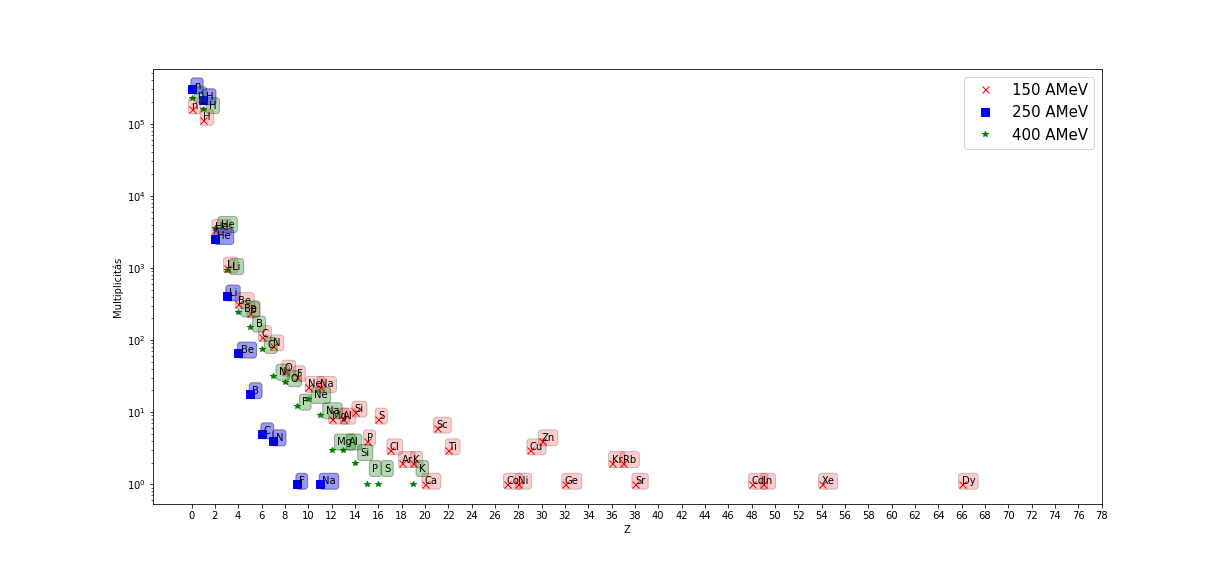
\includegraphics[width=1\textwidth]{./chemical.png}
\caption{Kémiai összetétel 150, 250 és 400 AMeV-en}
\end{figure}

\vspace{5mm}

\par Jól látható, hogy a kis rendszámú magok aránya nagyon magas, de megfigyelhető $C, O, B, Be, Na, F$ is kis mennyiségben. Ezek mind a természetben megtalálható izotópok. A várt módon egyre növekvő energián, egyre kevesebb mag alakul ki. A következő ábrákon külön külön is fel vannak tüntetve az egyes kémiai eloszlások.

\vspace{5mm}

\begin{figure}[H]
\begin{minipage}{\textwidth}
\centering
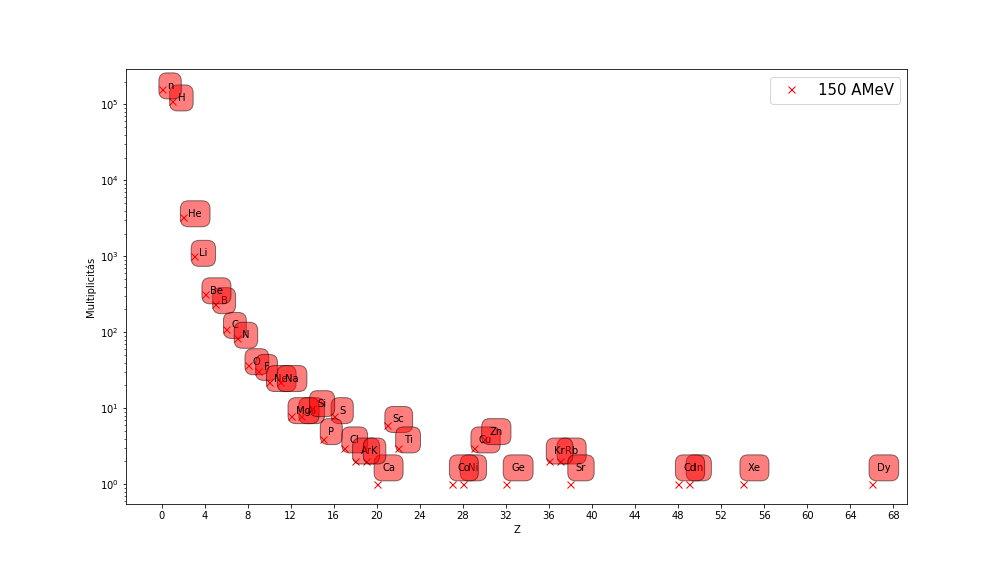
\includegraphics[width=0.7\textwidth]{./chemical150.png}
\caption{150 A MeV-en vett könnyű magok eloszlása 4$\pi$ tartományra integrálva}
\end{minipage}
\end{figure}
\begin{figure}[!htb]
\begin{minipage}{\textwidth}
\centering
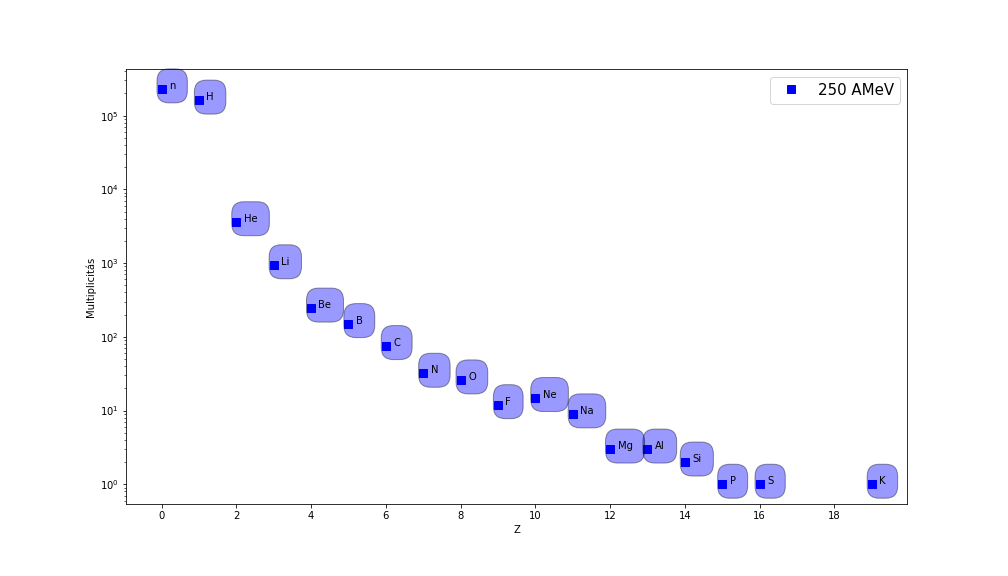
\includegraphics[width=0.7\textwidth]{./chemical250.png}
\caption{250 A MeV-en vett könnyű magok eloszlása 4$\pi$ tartományra integrálva}
\end{minipage}
\begin{minipage}{\textwidth}
\centering
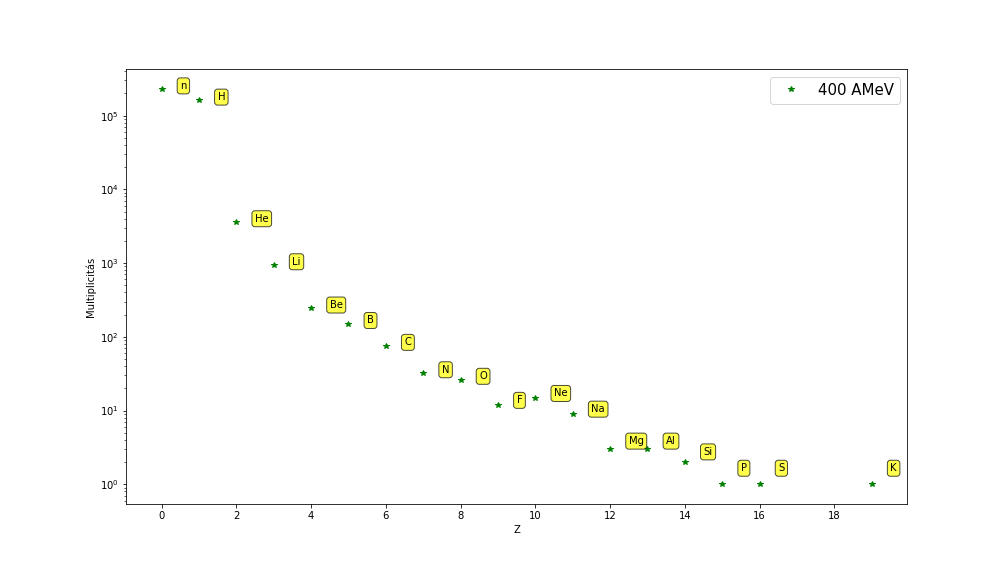
\includegraphics[width=0.7\textwidth]{./chemical400.png}
\caption{400 A MeV-en vett könnyű magok eloszlása 4$\pi$ tartományra integrálva}
\end{minipage}
\end{figure}

\section{ Eredmények összehasonlítása}

\vspace{5mm}

\par Most, hogy meghatároztam a klaszterek között a valós magokat érdemes a korábbi illesztést újra elvégezni,hogy ténylegesen össze tudjam hasonlítani a $FOPI$ által közölt adatokkal. Véve a közepes magokat és kihagyva a könnyű magokat és a $^{8}Be$-at, hiszen az nagyon hamar két $\alpha$-részecskére bomlik mielőtt ténylegesen elérné a detektort. Tehát ismét $M = N\cdot e^{-\lambda Z}$ illesztést végzek Z $\in$ [3] $\cup$ [5,12] tartományon. Hiszen a $Li$-magok nagy mennyiségben elérik a detektort. A könnyű magokat $Z = 0, 1, 2$ az \cite{REISDORF1997493}-höz hasonlóan kihagytam. 

\vspace{5mm}

\par Az illesztésből kapott $\lambda$ paramétereket és a \cite{REISDORF1997493} $\lambda$ paramétereit az alábbi táblázatban és az azt követő ábrákon is feltüntetem.

\vspace{5mm}

\begin{center}
\begin{tabular}{|c|c|c|}
\hline
E [AMeV] & $\lambda_{\text{saját}}$ & $\lambda_{FOPI}$ \\
\hline
150 & (0.697 $\pm$ 0.022) & (0.625 $\pm$ 0.010)\\
\hline
250  & (0.883 $\pm$ 0.026) & (0.908 $\pm$ 0.012)\\
\hline
400 & (1.543 $\pm$ 0.046) & (1.170 $\pm$ 0.018) \\
\hline
\end{tabular}
\end{center}

\vspace{5mm}

\begin{figure}[H]
\begin{minipage}{\textwidth}
\centering
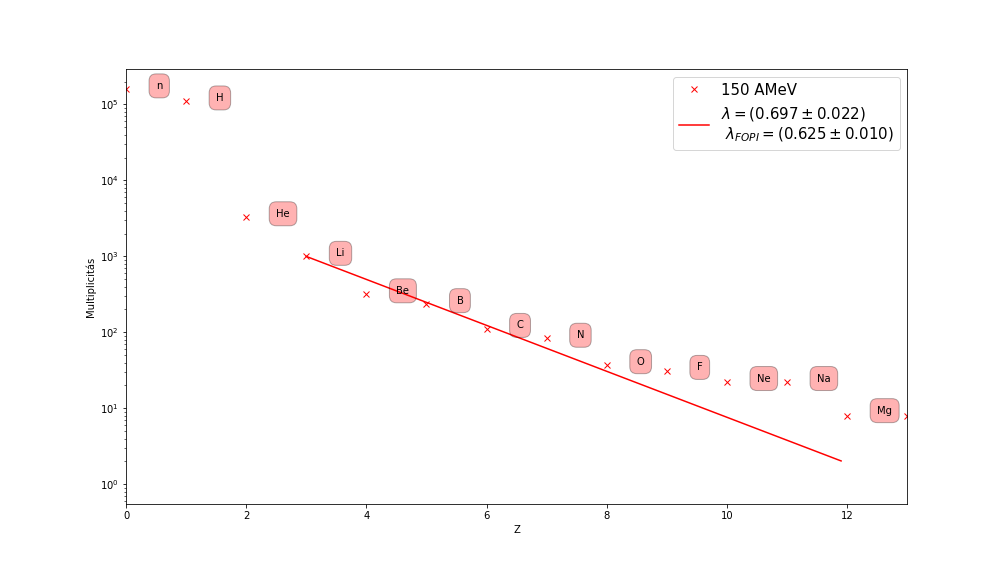
\includegraphics[width=\textwidth]{./FOPI150.png}
\caption{150 A MeV-en vett könnyű magok eloszlása, 4$\pi$ tartományra integrálva}
\end{minipage}
\end{figure}
\begin{figure}[H]
\begin{minipage}{\textwidth}
\centering
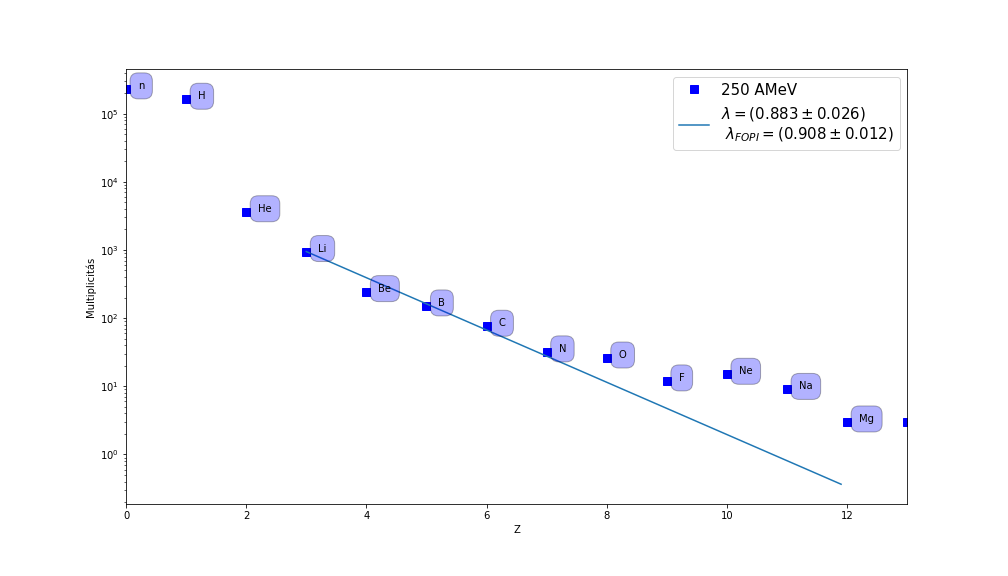
\includegraphics[width=\textwidth]{./FOPI250.png}
\caption{250 A MeV-en vett könnyű magok eloszlása, 4$\pi$ tartományra integrálva}
\end{minipage}
\end{figure}
\begin{figure}[H]
\begin{minipage}{\textwidth}
\centering
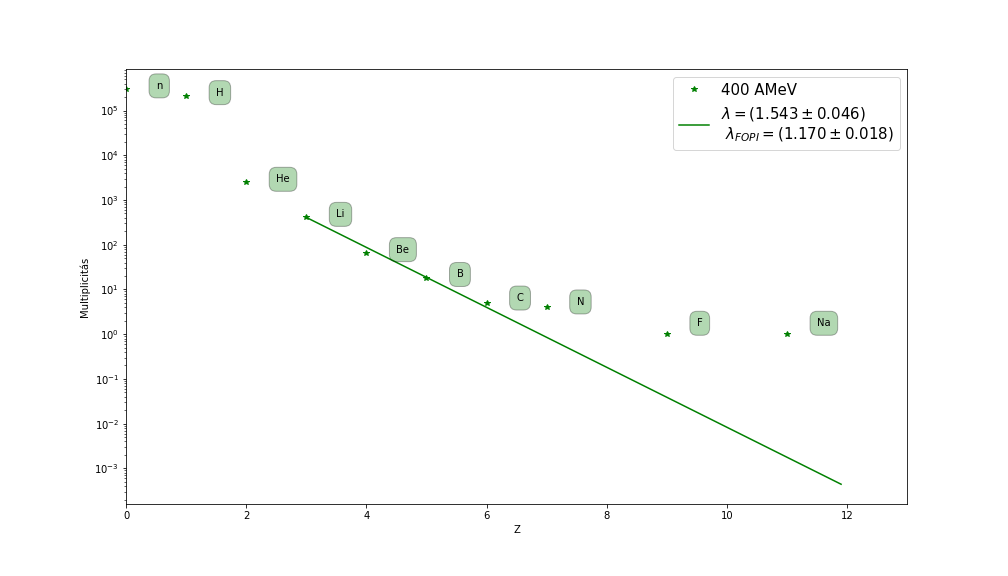
\includegraphics[width=\textwidth]{./FOPI400.png}
\caption{400 A MeV-en vett könnyű magok eloszlása, 4$\pi$ tartományra integrálva}
\end{minipage}
\end{figure}

\vspace{5mm}

\par Látható, hogy az illesztett görbék a nagyobb közepes magokra már nem jól illeszkednek. Vizsgálva, hogy ez hogyan függ $p_{0}$ értékétől el kellett végeznem ugyanezeket az illesztéseket, $p_{0}$ különböző értékérire. Míg korábban önkényesen $p_{0} = 60 ~MeV/c$-t vettem klaszterező paraméternek, most megpróbáltam megkeresni azt a klaszterező paramétert ami a legjobban illeszkedik a mérési adatokra. Jól látható továbbá az is, hogy a valós magokra való szűrés milyen nagy mértékben javította a korábbi illesztési adatokat. 

\vspace{5mm}

\begin{center}
\begin{tabular}{|c|c|c|c|c|}
\hline
E [AMeV] & $\lambda_{\text{saját}}$ & $\lambda_{\text{saját}}$ & $\lambda_{\text{saját}}$& $\lambda_{FOPI}$\\
\hline
150 & (1.001 $\pm$ 0.065)&(0.697 $\pm$ 0.022) & (0.795 $\pm$ 0.030) &(0.625 $\pm$ 0.010)\\
\hline
250  & (1.281 $\pm$ 0.018)&(0.883 $\pm$ 0.026) & (0.759 $\pm$ 0.026) &(0.908 $\pm$ 0.012)\\
\hline
400 & - &(1.543 $\pm$ 0.046) & (0.990 $\pm$ 0.014) &(1.170 $\pm$ 0.018) \\
\hline
- & $p_{0} = 50 ~MeV/c$ & $p_{0} = 60 ~MeV/c$&  $p_{0} = 70 ~MeV/c$  & - \\
\hline
\end{tabular}
\end{center}

\vspace{5mm}

\par $p_{0} = 50 ~MeV/c$-nél nem volt elég pont a függvényillesztéshez így az üresen maradt. Ezek az adatok jól szemléltetik, hogy a legtöbb magot létrehozó $p_{0}$ paraméter illeszkedik legjobban a mért adatokra. A legnagyobb energiás adat kiugró, ennek okát még keresni kell.

\vspace{5mm}

\begin{figure}[H]
\begin{minipage}{\textwidth}
\centering
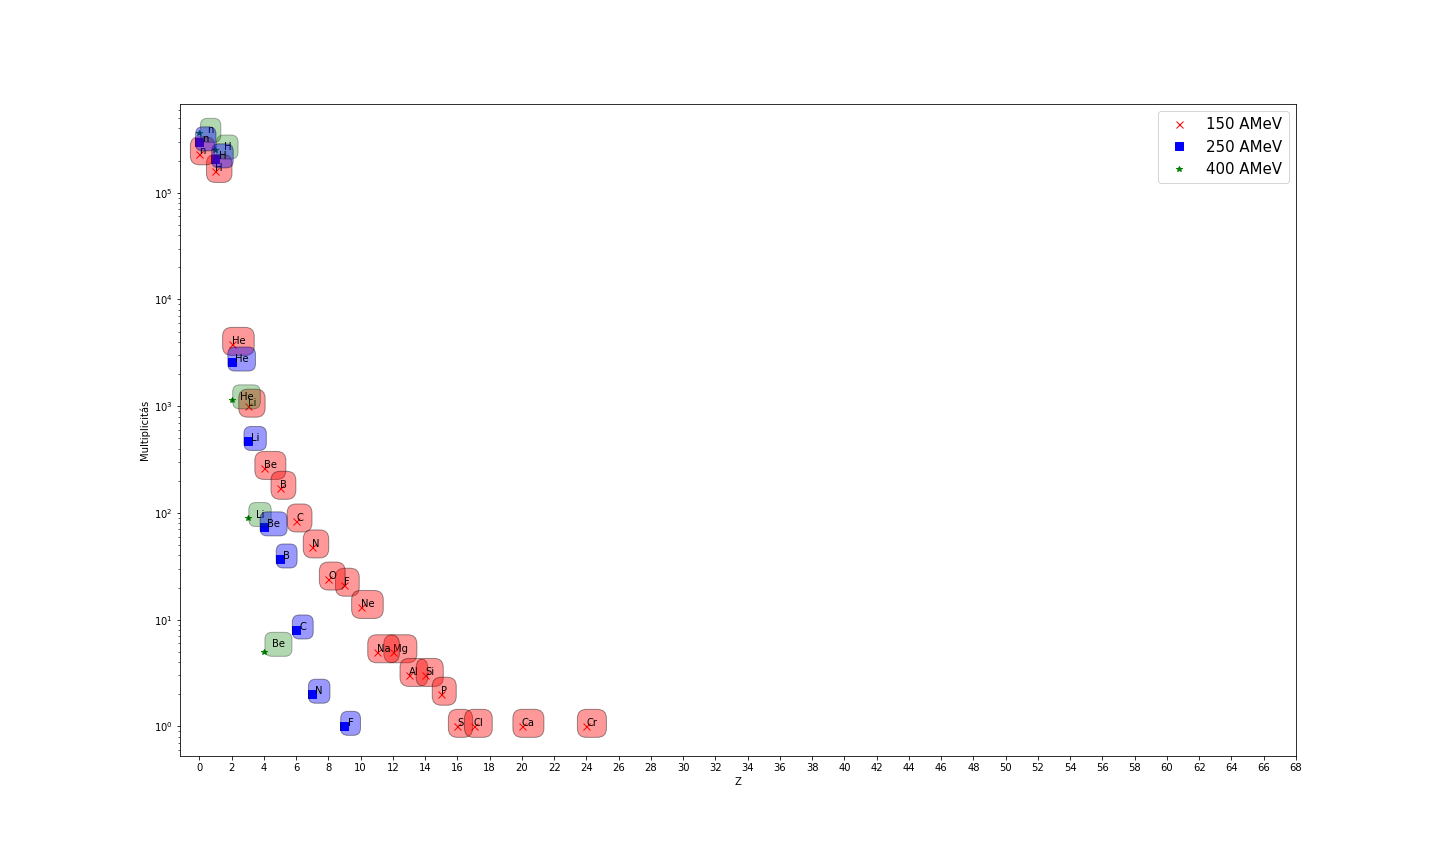
\includegraphics[width=0.9\textwidth]{./chemical_005.png}
\caption{$p_{0} = 50 ~MeV/c$ - kémiai eloszlás: a korábbihoz képest drasztikusan lecsökkent az összes klaszterek száma}
\end{minipage}
\end{figure}
\begin{figure}[H]
\begin{minipage}{\textwidth}
\centering
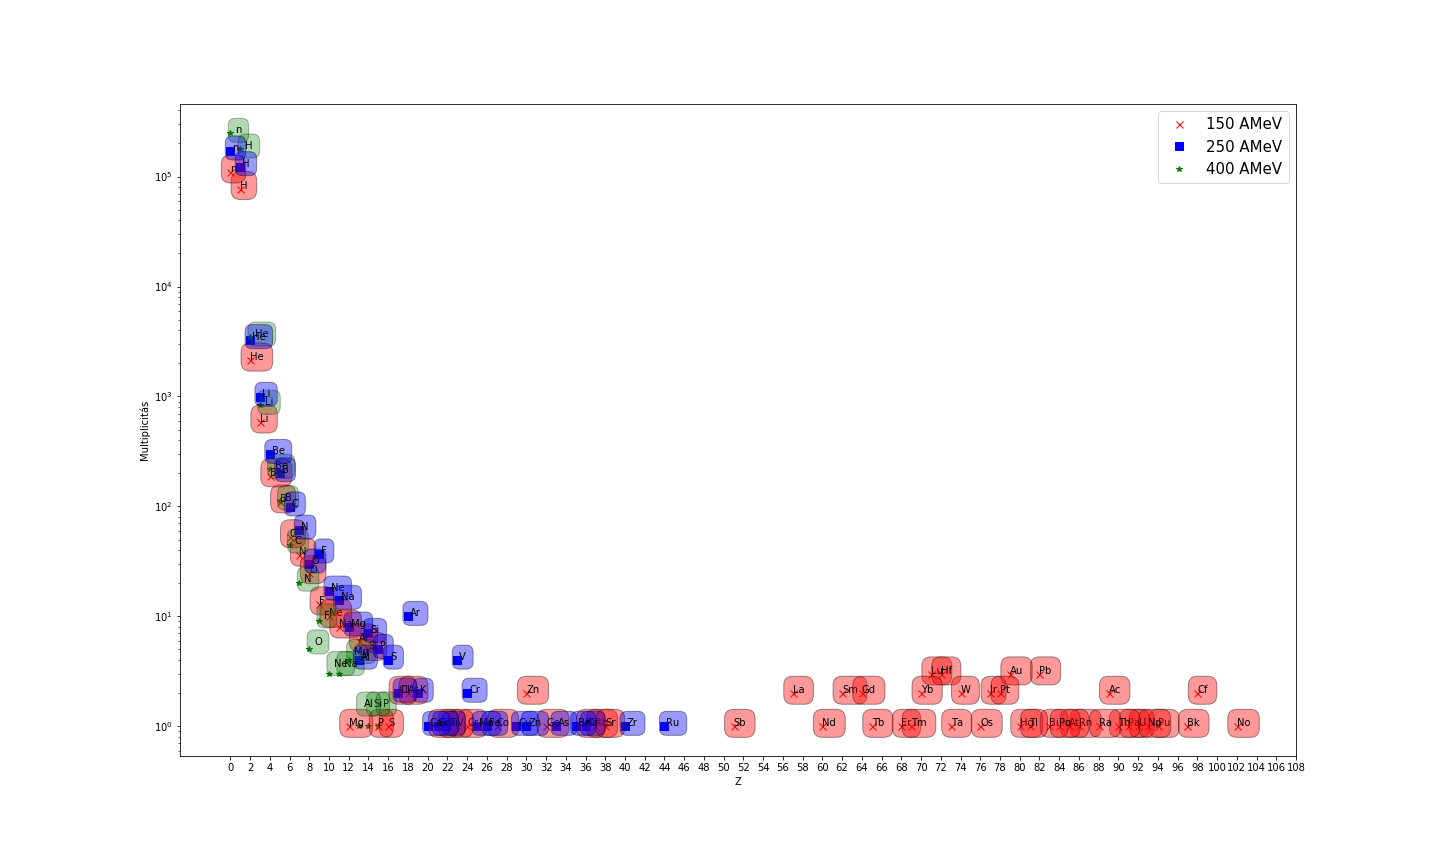
\includegraphics[width=0.9\textwidth]{./chemical_007.png}
\caption{$p_{0} = 70 ~MeV/c$ - kémiai eloszlás: kis energián sok különböző magot kaptam, viszont multiplicitásuk elenyésző}
\end{minipage}
\end{figure}

\vspace{5mm}

\section{ Összegzés}

\vspace{5mm}

\par A koaleszcencia modell kidolgozása során megismerkedtem rengeteg mostani kutatással, amely e témában tevékenykedik és az eredményeikkel összehasonlítható és mérési eredményekre részben illeszkedő rutint dolgoztam ki. Ez a későbbiekben használható lesz a témavezetőm által kidolgozott szimulációs kód részeként is.
\vspace{2mm} 
\par Az eredményeim közé tartozik, hogy egy a FOPI mérésekkel részben összehasonlítható algoritmust hoztam létre, amely során vizsgáltam a koaleszcencia modell helyességét már meglévő adatokon kvalitatíve és kvantitatíve. Az összehasonlítás természetesen nem teljesen pontos, hiszen a FOPI az ERAT mennyiséget választotta az események szortírozására, míg én csak centrális eseményekkel dolgoztam.
\vspace{2mm}
\par A kezdeti célkitűzéseimet elértem, hiszen képes voltam reprodukálni az alacsonyabb energiákon (150 AMeV, 250 AMeV) hibahatáron belül a mért eredményeket, valamint a jobb átláthatóság végett a korábbi mérések mintájára készítettem el az ábráimat, illesztéseimet.

\newpage

\bibliographystyle{plain}

\bibliography{references}

\end{document}